\documentstyle[11pt,epsfig,fancybox,semcolor,semlayer,doublespace,portrait]
{seminar}
\input clp_utils

% The following strings are needed by the title page and 
% page style definitions in map_utils.tex
\newcommand{\talktitle}[0]{{\sc Beamgas} and a Table of Background Systematics (Finally!)}
\newcommand{\fmttitle}[0]{}
\newcommand{\conftitle}[0]{CLEO PTA}
\newcommand{\myname}[0]{Jim Pivarski}
\newcommand{\affila}[0]{Cornell University}
\newcommand{\talkdate}[0]{March 7, 2002}

\pagestyle{conference}   % From clp_utils.tex

% slide magnification
\slidesmag 1

%%%%%%%%%%%%%%%%%%%%%%%%%%%%%%%%%%%%%%%%%%%%%%%%%%%%%%%%%%%%%%%%%%%%%%%%%%%
% Start document
\begin{document}

% Set page size
\slideheight 7.0in
\slidewidth 8.8in 

% Set array stretch
\renewcommand{\arraystretch}{0.3}
\renewcommand{\slidetopmargin}{0.4in}
\renewcommand{\slidebottommargin}{0.9in}


%%%%%%%%%%%%%%%%%%%%%%%%%%%%%%%%%%%%%%%%%%%%%%%%%%%%%%%%%%%%%%%%%%%%%%%%%%%

\begin{slide*}

\slideframe{}
\slideframe*[\dkblue]{Oval}

\begin{center}
\vspace{4 cm}
{\Huge \black {\sc Beamgas} \\ and a \\ Table of Background Systematics \\ \mbox{ } \\ (Finally!) } \\
\vspace{1 cm}
{\LARGE \black	Jim Pivarski } \\
% \vspace{0.25 cm}
% {\LARGE	Ritchie Patterson } \\
% \vspace{0.25 cm}
% {\LARGE	Karl Berkelman } \\
\vspace{2 cm}
\conftitle \\
{\large \black \talkdate}

\end{center}

\end{slide*}

% %%%%%%%%%%%%%%%%%%%%%%%%%%%%%%%%%%%%%%%%%%%%%%%%%%%%%%%%%%%%%%%%%%%%%%%%%%%

\begin{slide*}

\slideframe{}
\slideframe*[\dkblue]{Oval}
\huge
\heading{Review of Cuts}

\begin{minipage}[t]{\linewidth}
\large

\begin{tabular}{c c}

\begin{minipage}{0.45\linewidth}
\begin{itemize}

  \item Hadron Subcollection Cuts \\
        \hspace{1 cm} \small (keep 95\% of signal, 0.2\% of bkgnd)

\end{itemize}
\end{minipage} &
\begin{minipage}{0.5\linewidth}
\begin{itemize}

  \item Closest Intersection and Event Z Cuts \\
        \hspace{1 cm} \small (keep 99.4\% of signal, 43\% of bkgnd)

\end{itemize}
\end{minipage}

\end{tabular}

\begin{center}
  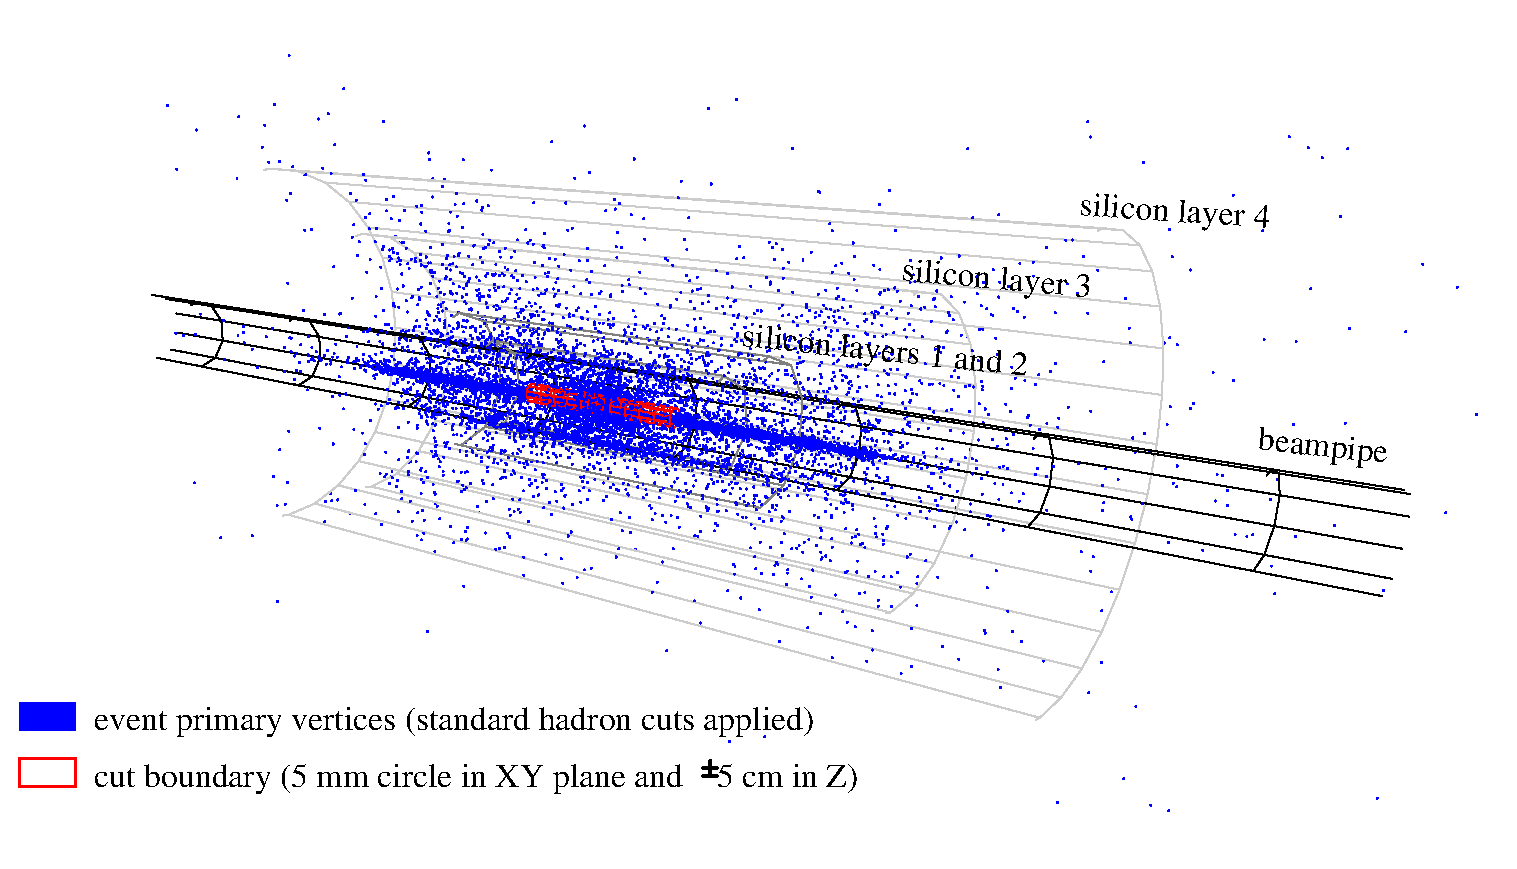
\includegraphics[width=0.9\linewidth]{cuts_illustration4.eps}
\end{center}

\begin{center}
  \includegraphics[width=0.9\linewidth]{cuts_illustration5.eps}
\end{center}

(Cuts publicly available via {\tt BeamGasFilterProc}.)

\end{minipage}

\end{slide*}

%%%%%%%%%%%%%%%%%%%%%%%%%%%%%%%%%%%%%%%%%%%%%%%%%%%%%%%%%%%%%%%%%%%%%%%%%%%

% %%%%%%%%%%%%%%%%%%%%%%%%%%%%%%%%%%%%%%%%%%%%%%%%%%%%%%%%%%%%%%%%%%%%%%%%%%%

\begin{slide*}

\slideframe{}
\slideframe*[\dkblue]{Oval}
\huge
\heading{Review of Cuts}

\begin{minipage}[t]{\linewidth}
\large

{\huge What about cutting on neutral energy?}

\begin{center}
\begin{tabular}{p{0.45\linewidth} p{1cm} p{0.45\linewidth}}
  \begin{minipage}{\linewidth}
    \begin{center}
      \begin{minipage}{0.95\linewidth}
        {\bf Claim:} \\ Beamgas has zero neutral energy \\
      \end{minipage}
      \includegraphics[width=0.75\linewidth]{neutral_energy2.eps} \\
      {\Large \bf FALSE!}
    \end{center}
  \end{minipage} & &
  \begin{minipage}{\linewidth}
    \begin{center}
      \begin{minipage}{0.95\linewidth}
        {\bf \mbox{ }} \\ Hadronic data does not \\
      \end{minipage}
      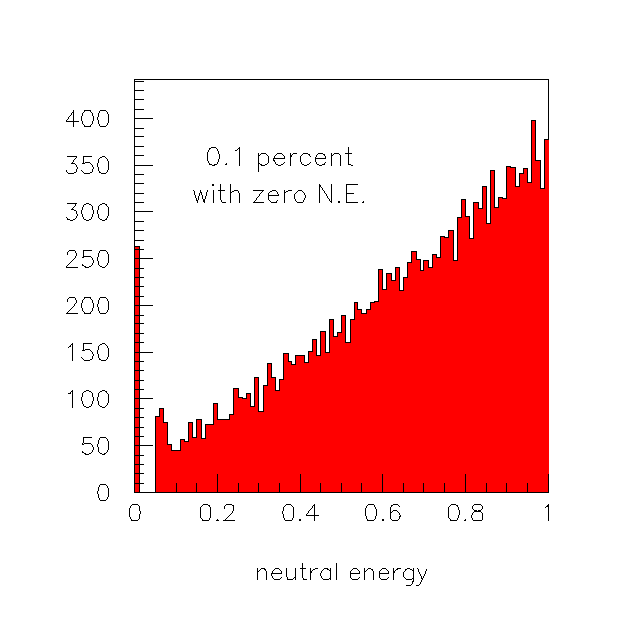
\includegraphics[width=0.75\linewidth]{neutral_energy1.eps} \\
      {\bf \Large TRUE.}
    \end{center}
  \end{minipage} \\
\end{tabular}
\end{center}

\vspace{0.5cm}

\begin{center}
\begin{tabular}{p{0.45\linewidth} p{1cm} p{0.45\linewidth}}
  \begin{minipage}{\linewidth}
    I did track-shower matching incorrectly.  Real beamgas does have
    some neutral energy.
    \begin{center}
      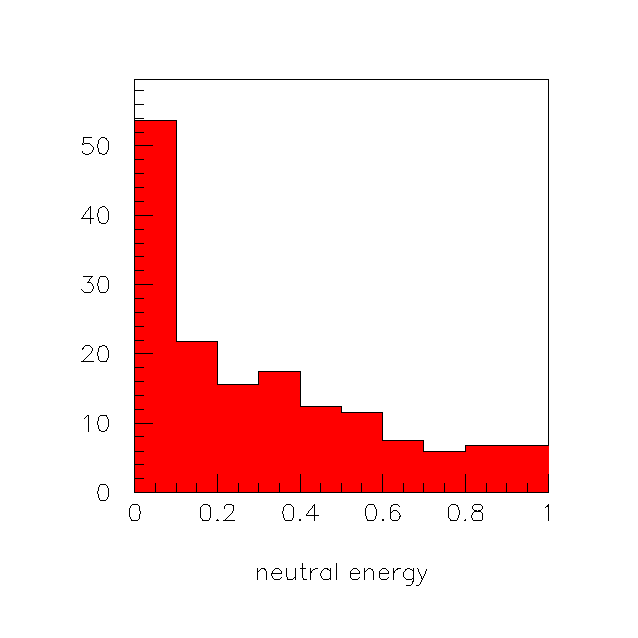
\includegraphics[width=0.75\linewidth]{neutral_energy3.eps} \\
      {\bf \Large Can't make a clean cut.}
    \end{center}
  \end{minipage} & & \\
\end{tabular}
\end{center}

\end{minipage}

\end{slide*}

%%%%%%%%%%%%%%%%%%%%%%%%%%%%%%%%%%%%%%%%%%%%%%%%%%%%%%%%%%%%%%%%%%%%%%%%%%%

% %%%%%%%%%%%%%%%%%%%%%%%%%%%%%%%%%%%%%%%%%%%%%%%%%%%%%%%%%%%%%%%%%%%%%%%%%%%

\begin{slide*}

\slideframe{}
\slideframe*[\dkblue]{Oval}
\huge
\heading{If You Can't Cut Them, Count Them}

\begin{minipage}[t]{\linewidth}
\large

{\bf Procedure:}
\begin{enumerate}

  \item Apply all cuts except the Z cut

  \item Count beamgas events in 5 cm $< |z| <$ 20 cm

  \item Cut on Z

  \item Use Single-Beam data to project into $|z| <$ 5 cm region, to
  determine how many beamgas events pass cuts

\end{enumerate}

\vspace{-0.5cm}

\begin{center}
  \includegraphics[width=0.85\linewidth]{determine_factor.eps}
\end{center}

This algorithm has been added to {\tt BeamGasFilterProc}.

\end{minipage}

\end{slide*}

%%%%%%%%%%%%%%%%%%%%%%%%%%%%%%%%%%%%%%%%%%%%%%%%%%%%%%%%%%%%%%%%%%%%%%%%%%%

% %%%%%%%%%%%%%%%%%%%%%%%%%%%%%%%%%%%%%%%%%%%%%%%%%%%%%%%%%%%%%%%%%%%%%%%%%%%

\begin{slide*}

\slideframe{}
\slideframe*[\dkblue]{Oval}
\huge
\heading{If You Can't Cut Them, Count Them}

\begin{minipage}[t]{\linewidth}
\Large

Data events in 5 cm $< |z| <$ 20 cm {\it are} beamgas events!

\vspace{0.65cm}

\begin{center}
  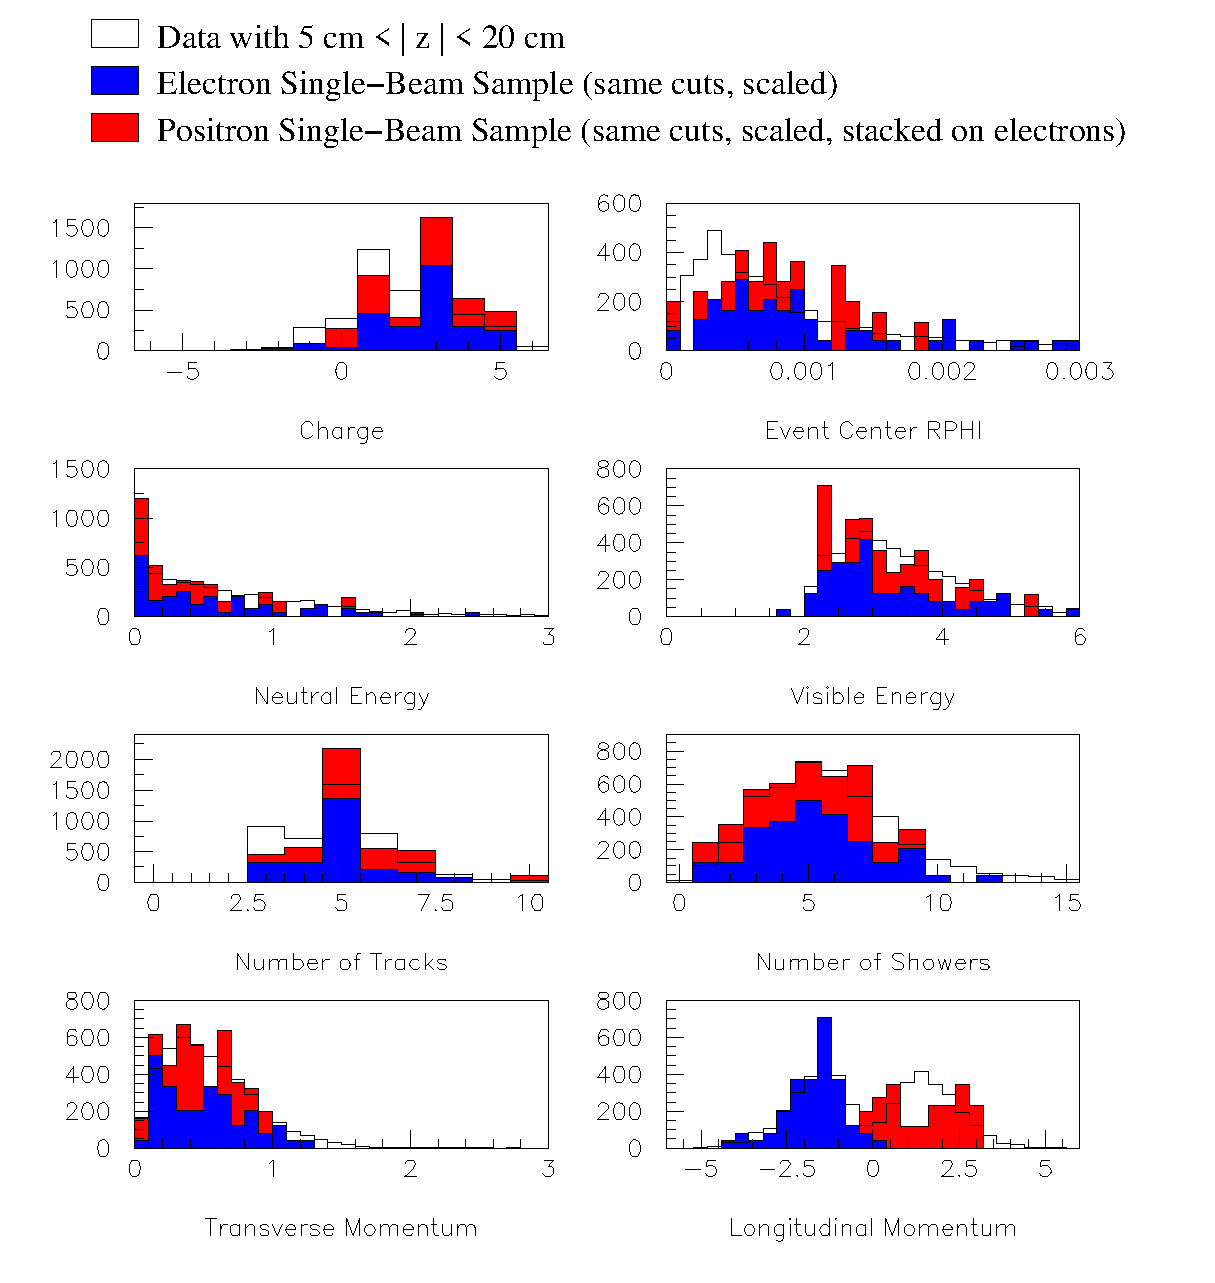
\includegraphics[width=\linewidth]{check_beamgas2.eps}
\end{center}

\end{minipage}

\end{slide*}

%%%%%%%%%%%%%%%%%%%%%%%%%%%%%%%%%%%%%%%%%%%%%%%%%%%%%%%%%%%%%%%%%%%%%%%%%%%

%% % %%%%%%%%%%%%%%%%%%%%%%%%%%%%%%%%%%%%%%%%%%%%%%%%%%%%%%%%%%%%%%%%%%%%%%%%%%%

\begin{slide*}

\slideframe{}
\slideframe*[\dkblue]{Oval}
\huge
\heading{Toward a Systematics Table}

\begin{minipage}[t]{\linewidth}
\Large

Uncertainty in area due to\ldots

\begin{itemize}

  \item Beamgas = 0.060\% at $\Upsilon$(1S) and 0.015\% at $\Upsilon$(3S)

  \item Beamwall $\approx$ Beamgas / 10 = 0.006\%

  \item Cosmics $\approx$ Beamgas / 15 = 0.004\%

\end{itemize}

\vspace{-0.5cm}

\begin{center}
  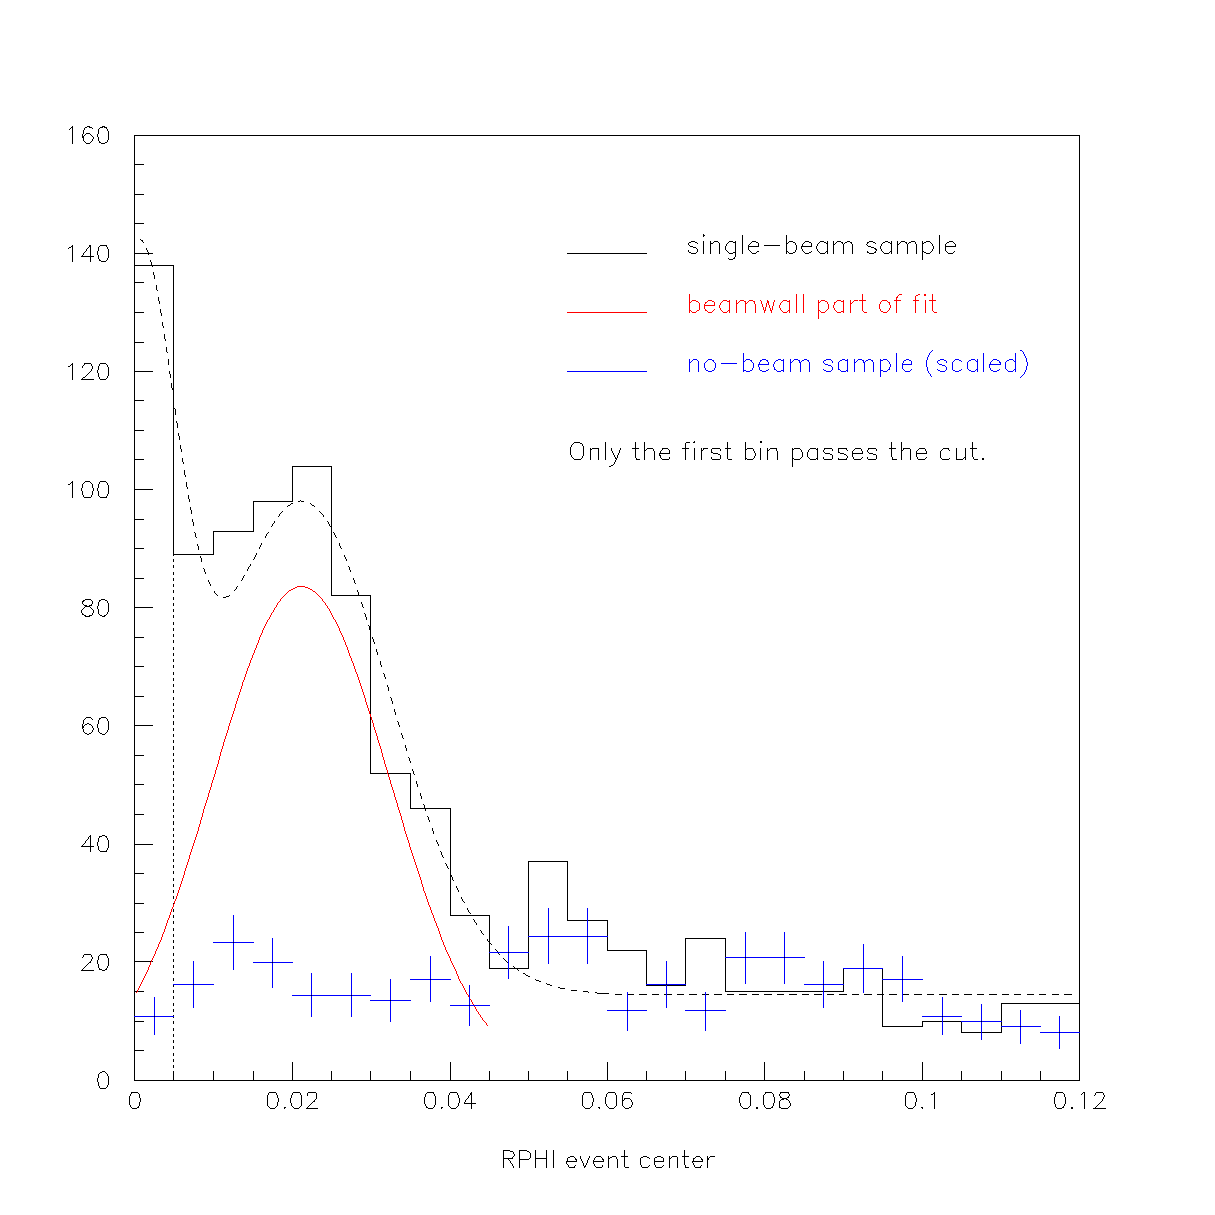
\includegraphics[width=0.9\linewidth]{cosmics_vs_beamgas.eps}
\end{center}

\end{minipage}

\end{slide*}

% %%%%%%%%%%%%%%%%%%%%%%%%%%%%%%%%%%%%%%%%%%%%%%%%%%%%%%%%%%%%%%%%%%%%%%%%%%%

\begin{slide*}

\slideframe{}
\slideframe*[\dkblue]{Oval}
\huge
\heading{Further Toward a Systematics Table}

\begin{minipage}[t]{\linewidth}
\large

The hadronic cross-section is contaminated by about 0.7\% tau pair events:

\[
\frac{e^+ e^- \to \Upsilon \to \tau^+ \tau^-}{\mbox{hadronic events}} = \hspace{10cm}
\]
\vspace{-1cm}
\[
\hspace{2.5cm} =
\frac{\epsilon(\tau^+ \tau^-)}{\epsilon(\mbox{hadrons})} \cdot
\frac{1}{1/{\mathcal B}_{\mu\mu} - 3} =
\frac{0.2493}{0.9287} \cdot \left\{ \begin{array}{c c c}
0.0268 & & \mbox{for } \Upsilon(\mbox{1S}) \\
0.0136 & & \mbox{for } \Upsilon(\mbox{2S}) \\
0.0191 & & \mbox{for } \Upsilon(\mbox{3S}) \\
\end{array} \right.
\]

\vspace{-1cm}

\begin{center}
  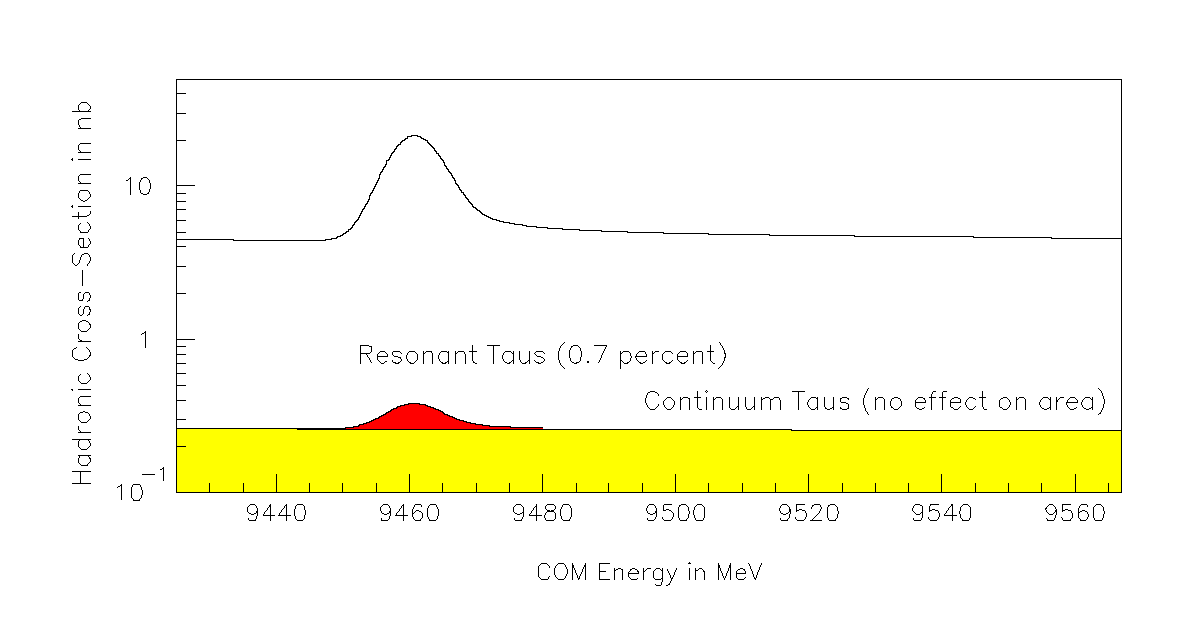
\includegraphics[width=\linewidth]{plot_taus.eps}
\end{center}

\vspace{-0.5cm}

Include it in the fit function to calculate interference terms of

{ \Large
\[ \left| \begin{array}{c c c}
    \mbox{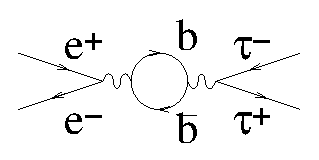
\includegraphics[height=1cm]{tau_interference.eps}} &
    \mbox{\includegraphics[height=1cm]{plus.eps}} &
    \mbox{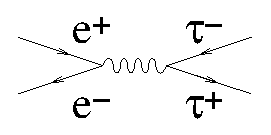
\includegraphics[height=1cm]{tau_interference2.eps}} \\
\end{array} \right|^2
\] }
(Interference is 40\% of $e^+ e^- \to \Upsilon \to \tau^+ \tau^-$ cross-section.)

\vspace{0.5cm}

\begin{center}
  \begin{tabular}{r | c | c}
    & Effect on $\Upsilon(\mbox{1S})$ area & Effect on $\Upsilon(\mbox{3S})$ area \\\hline
    Vary ${\mathcal B}_{\mu\mu}$ by 1 PDG $\sigma$ & 0.018\% & 0.038\% \\
    Turn interference on and off & 0.089\% & 0.0043\% \\
    Let continuum tau phase be 1$^\circ$ & 0.0016\% & 0.0022\% \\
  \end{tabular}
\end{center}

\end{minipage}

\end{slide*}

%% % %%%%%%%%%%%%%%%%%%%%%%%%%%%%%%%%%%%%%%%%%%%%%%%%%%%%%%%%%%%%%%%%%%%%%%%%%%%

\begin{slide*}

\slideframe{}
\slideframe*[\dkblue]{Oval}
\huge
\heading{{\Large Yet Further} Toward a Systematics Table}

\begin{minipage}[t]{\linewidth}
\large

The hadronic part can interfere with the $q\bar{q}$ background
(1.7\% $\frac{\mbox{interference}}{\mbox{cross-section}}$):

\begin{center}
  \begin{tabular}{l r}
    \begin{minipage}{0.25\linewidth}
      \includegraphics[width=\linewidth]{bigyint_lineshape.eps}
    \end{minipage} &
    \begin{minipage}{0.6\linewidth}
      \begin{center}
        \begin{tabular}{r | c | c}
          & $\Upsilon(\mbox{1S})$ & $\Upsilon(\mbox{3S})$ \\\hline
          Double $q\bar{q}$ interference & 0.56\% & 0.0044\% \\
          Let continuum $q\bar{q}$ phase be 1$^\circ$ & 0.029\% & 0.028\% \\
        \end{tabular}
      \end{center}
    \end{minipage} \\
  \end{tabular}
\end{center}

\vspace{1cm}
The two-photon component of the background (3.3\%) scales as $\log s$:

\begin{center}
  \begin{tabular}{l r}
    \begin{minipage}{0.25\linewidth}
      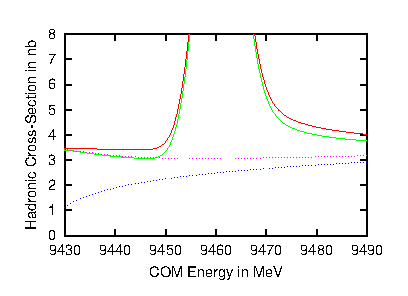
\includegraphics[width=\linewidth]{fakedback_lineshape.eps}
    \end{minipage} &
    \begin{minipage}{0.6\linewidth}
      \begin{center}
        \begin{tabular}{r | c | c}
          & $\Upsilon(\mbox{1S})$ & $\Upsilon(\mbox{3S})$ \\\hline
	  Turn off two-photon component & 0.011\% & 0.014\% \\
	  Let it be 10\% of continuum data & 0.021\% & 0.033\% \\
        \end{tabular}
      \end{center}
    \end{minipage} \\
  \end{tabular}
\end{center}

\vspace{1cm}
Part of the background comes from ISR tails from $J/\psi$'s (1\%):

\begin{center}
  \begin{tabular}{l r}
    \begin{minipage}{0.25\linewidth}
      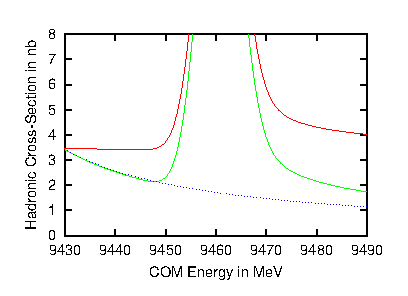
\includegraphics[width=\linewidth]{fakedback2_lineshape.eps}
    \end{minipage} &
    \begin{minipage}{0.6\linewidth}
      \begin{center}
        \begin{tabular}{r | c | c}
          & $\Upsilon(\mbox{1S})$ & $\Upsilon(\mbox{3S})$ \\\hline
	  Turn off/double tails & 0.00060\% & 0.025\% \\
        \end{tabular}
      \end{center}
    \end{minipage} \\
  \end{tabular}
\end{center}

\vspace{1cm}
Intrinsic width of resonance affects the peak height:

\begin{center}
  \begin{tabular}{l r}
    \begin{minipage}{0.25\linewidth}
      \includegraphics[width=\linewidth]{biggam_lineshape.eps}
    \end{minipage} &
    \begin{minipage}{0.6\linewidth}
      \begin{center}
        \begin{tabular}{r | c | c}
          & $\Upsilon(\mbox{1S})$ & $\Upsilon(\mbox{3S})$ \\\hline
	  Vary $\Gamma$ by 1 PDG $\sigma$ & 0.0043\% & 0.011\% \\
        \end{tabular}
      \end{center}
    \end{minipage} \\
  \end{tabular}
\end{center}

\end{minipage}

\end{slide*}

%% % %%%%%%%%%%%%%%%%%%%%%%%%%%%%%%%%%%%%%%%%%%%%%%%%%%%%%%%%%%%%%%%%%%%%%%%%%%%

\begin{slide*}

\slideframe{}
\slideframe*[\dkblue]{Oval}
\huge
\heading{The Systematics Table}

\begin{minipage}[t]{\linewidth}
\large

Uncertainty in area is proportional to uncertainty in
$\Gamma(\mbox{hadrons}) \times \Gamma(e^+ e^-)/\Gamma_{\mbox{total}}$

\vspace{0.5cm}

\begin{center}
  \begin{tabular}{l c c}
    & $\Upsilon(\mbox{1S})$ Area Uncertainty & $\Upsilon(\mbox{3S})$ Area Uncertainty \\\hline

    Beamgas  			      & 0.060\%   & 0.015\% \\
    Beamwall 			      & 0.006\%   & 0.002\% \\
    Cosmics  			      & 0.004\%   & 0.001\% \\
    Two-photon                        & 0.021\%   & 0.033\% \\
    $J/\psi$ and $\Upsilon$ ISR tails & 0.00060\% & 0.025\% \\
    $\Upsilon \to \tau^+ \tau^-$      & 0.018\%   & 0.038\% \\
    $\tau$-pair interference 	      & 0.089\%   & 0.038\% \\
    $q\bar{q}$ interference  	      & 0.56\%    & 0.028\% \\
    Finite $\Gamma$          	      & 0.00043\% & 0.011\% \\\hline
    Sum in quadrature        	      & 0.57\%    & 0.076\% \vspace{0.5cm}\\

    Luminosity                        & $\sim$2\%    & $\sim$2\%    \\
    Acceptance                        & $\sim$0.5\%  & $\sim$0.5\%  \\
    Energy Calibration                & $\sim$0.75\% & $\sim$0.75\% \vspace{0.5cm}\\

    Statistical uncertainty           & 0.18\%       & 0.61\% \\\hline
    Grand Total                       & $\sim$2.3\%  & $\sim$2.3\%  \vspace{0.5cm}\\

    PDG Best Value                    & \hspace{1.5cm} 3.3\% {\scriptsize \sc (Novo '96)} & \hspace{1.5cm} 9.4\% {\scriptsize \sc (Cleo '84)} \\
    PDG Average                       & 2.2\%            & {\it same}

  \end{tabular}
\end{center}

\end{minipage}

\end{slide*}

% %%%%%%%%%%%%%%%%%%%%%%%%%%%%%%%%%%%%%%%%%%%%%%%%%%%%%%%%%%%%%%%%%%%%%%%%%%%

\begin{slide*}

\slideframe{}
\slideframe*[\dkblue]{Oval}
\huge
\heading{The Almost--Final Fits!}

\begin{minipage}[t]{\linewidth}
\large

\vspace{0.1cm}

All they need now is an efficiency correction, and a better
measurement of luminosity.

\vspace{0.1cm}

\begin{center}
  \begin{tabular}{c p{1cm} c}
    Sample $\Upsilon(\mbox{1S})$ Fit & & Sample $\Upsilon(\mbox{3S})$ Fit \\
    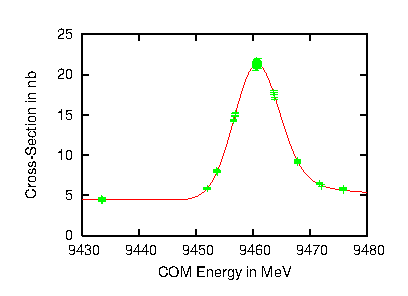
\includegraphics[width=0.4\linewidth]{y1s_lineshape.eps} & & 
      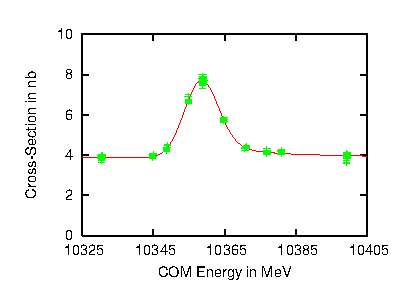
\includegraphics[width=0.4\linewidth]{y3s_lineshape.eps} \\
    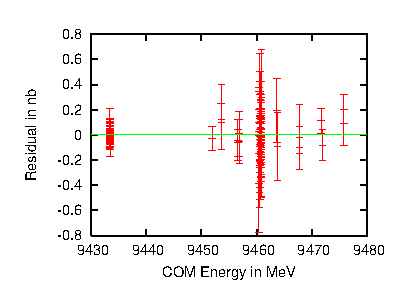
\includegraphics[width=0.4\linewidth]{y1s_resid.eps} & & 
      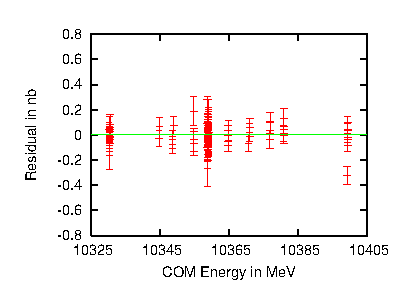
\includegraphics[width=0.4\linewidth]{y3s_resid.eps} \\
    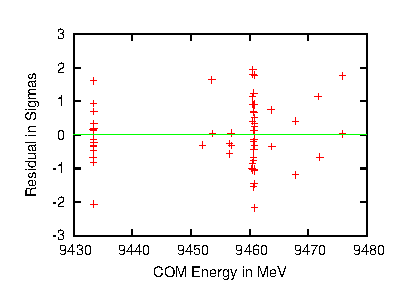
\includegraphics[width=0.4\linewidth]{y1s_normresid.eps} & & 
      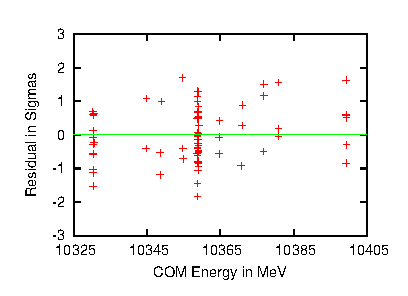
\includegraphics[width=0.4\linewidth]{y3s_normresid.eps} \\
  \end{tabular}
\end{center}

\vspace{0.1cm}

\end{minipage}

\end{slide*}

% %%%%%%%%%%%%%%%%%%%%%%%%%%%%%%%%%%%%%%%%%%%%%%%%%%%%%%%%%%%%%%%%%%%%%%%%%%%

\begin{slide*}

\slideframe{}
\slideframe*[\dkblue]{Oval}
\huge
\heading{Conclusions}

\begin{minipage}[t]{\linewidth}
\Large

\vspace{0.5cm}

\begin{itemize}

  \item All background systematics are insignificant, except possibly for 
  $q\bar{q}$ interference in the $\Upsilon(\mbox{1S})$ (0.56\%).

  \vspace{1cm}

  \item Even with current (conservative) estimates for remaining
  systematics, this measurement is competitive.

  \vspace{1cm}

  \item If you use the default cuts, {\tt BeamGasFilterProc} will now
  count surviving beamgas events for you.  (Probably still in
  development, though.)

  \vspace{1cm}

  \item The neutral energy cut is not so efficient at eliminating
  beamgas as I had previously claimed.

  \vspace{1cm}

  \item Thank you Karl Berkelman for the interference calculations,
  and Steve Dytman and Surik Mehrabyan for the two-photon measurement!

\end{itemize}

\end{minipage}

\end{slide*}

% %%%%%%%%%%%%%%%%%%%%%%%%%%%%%%%%%%%%%%%%%%%%%%%%%%%%%%%%%%%%%%%%%%%%%%%%%%%

%% \begin{slide*}

%% \slideframe{}
%% \slideframe*[\dkblue]{Oval}
%% \huge
%% \heading{REPLACEME}

%% \begin{minipage}[t]{\linewidth}
%% \large

%% \begin{center}
%%   \includegraphics[width=\linewidth]{}
%% \end{center}

%% \end{minipage}

%% \end{slide*}

%% % %%%%%%%%%%%%%%%%%%%%%%%%%%%%%%%%%%%%%%%%%%%%%%%%%%%%%%%%%%%%%%%%%%%%%%%%%%%

%% \begin{slide*}

%% \slideframe{}
%% \slideframe*[\dkblue]{Oval}
%% \huge
%% \heading{REPLACEME}

%% \begin{minipage}[t]{\linewidth}
%% \large

%% \begin{center}
%%   \includegraphics[width=\linewidth]{}
%% \end{center}

%% \end{minipage}

%% \end{slide*}

%% % %%%%%%%%%%%%%%%%%%%%%%%%%%%%%%%%%%%%%%%%%%%%%%%%%%%%%%%%%%%%%%%%%%%%%%%%%%%

%% \begin{slide*}

%% \slideframe{}
%% \slideframe*[\dkblue]{Oval}
%% \huge
%% \heading{REPLACEME}

%% \begin{minipage}[t]{\linewidth}
%% \large

%% \begin{center}
%%   \includegraphics[width=\linewidth]{}
%% \end{center}

%% \end{minipage}

%% \end{slide*}

%% % %%%%%%%%%%%%%%%%%%%%%%%%%%%%%%%%%%%%%%%%%%%%%%%%%%%%%%%%%%%%%%%%%%%%%%%%%%%

%% \begin{slide*}

%% \slideframe{}
%% \slideframe*[\dkblue]{Oval}
%% \huge
%% \heading{REPLACEME}

%% \begin{minipage}[t]{\linewidth}
%% \large

%% \begin{center}
%%   \includegraphics[width=\linewidth]{}
%% \end{center}

%% \end{minipage}

%% \end{slide*}

%% % %%%%%%%%%%%%%%%%%%%%%%%%%%%%%%%%%%%%%%%%%%%%%%%%%%%%%%%%%%%%%%%%%%%%%%%%%%%

%% \begin{slide*}

%% \slideframe{}
%% \slideframe*[\dkblue]{Oval}
%% \huge
%% \heading{REPLACEME}

%% \begin{minipage}[t]{\linewidth}
%% \large

%% \begin{center}
%%   \includegraphics[width=\linewidth]{}
%% \end{center}

%% \end{minipage}

%% \end{slide*}

%% % %%%%%%%%%%%%%%%%%%%%%%%%%%%%%%%%%%%%%%%%%%%%%%%%%%%%%%%%%%%%%%%%%%%%%%%%%%%

%% \begin{slide*}

%% \slideframe{}
%% \slideframe*[\dkblue]{Oval}
%% \huge
%% \heading{REPLACEME}

%% \begin{minipage}[t]{\linewidth}
%% \large

%% \begin{center}
%%   \includegraphics[width=\linewidth]{}
%% \end{center}

%% \end{minipage}

%% \end{slide*}

%% % %%%%%%%%%%%%%%%%%%%%%%%%%%%%%%%%%%%%%%%%%%%%%%%%%%%%%%%%%%%%%%%%%%%%%%%%%%%

%% \begin{slide*}

%% \slideframe{}
%% \slideframe*[\dkblue]{Oval}
%% \huge
%% \heading{REPLACEME}

%% \begin{minipage}[t]{\linewidth}
%% \large

%% \begin{center}
%%   \includegraphics[width=\linewidth]{}
%% \end{center}

%% \end{minipage}

%% \end{slide*}

%% % %%%%%%%%%%%%%%%%%%%%%%%%%%%%%%%%%%%%%%%%%%%%%%%%%%%%%%%%%%%%%%%%%%%%%%%%%%%

%% \begin{slide*}

%% \slideframe{}
%% \slideframe*[\dkblue]{Oval}
%% \huge
%% \heading{REPLACEME}

%% \begin{minipage}[t]{\linewidth}
%% \large

%% \begin{center}
%%   \includegraphics[width=\linewidth]{}
%% \end{center}

%% \end{minipage}

%% \end{slide*}

%% % %%%%%%%%%%%%%%%%%%%%%%%%%%%%%%%%%%%%%%%%%%%%%%%%%%%%%%%%%%%%%%%%%%%%%%%%%%%

%% \begin{slide*}

%% \slideframe{}
%% \slideframe*[\dkblue]{Oval}
%% \huge
%% \heading{REPLACEME}

%% \begin{minipage}[t]{\linewidth}
%% \large

%% \begin{center}
%%   \includegraphics[width=\linewidth]{}
%% \end{center}

%% \end{minipage}

%% \end{slide*}

%% % %%%%%%%%%%%%%%%%%%%%%%%%%%%%%%%%%%%%%%%%%%%%%%%%%%%%%%%%%%%%%%%%%%%%%%%%%%%

%% \begin{slide*}

%% \slideframe{}
%% \slideframe*[\dkblue]{Oval}
%% \huge
%% \heading{REPLACEME}

%% \begin{minipage}[t]{\linewidth}
%% \large

%% \begin{center}
%%   \includegraphics[width=\linewidth]{}
%% \end{center}

%% \end{minipage}

%% \end{slide*}

%% % %%%%%%%%%%%%%%%%%%%%%%%%%%%%%%%%%%%%%%%%%%%%%%%%%%%%%%%%%%%%%%%%%%%%%%%%%%%

%% \begin{slide*}

%% \slideframe{}
%% \slideframe*[\dkblue]{Oval}
%% \huge
%% \heading{REPLACEME}

%% \begin{minipage}[t]{\linewidth}
%% \large

%% \begin{center}
%%   \includegraphics[width=\linewidth]{}
%% \end{center}

%% \end{minipage}

%% \end{slide*}

%% % %%%%%%%%%%%%%%%%%%%%%%%%%%%%%%%%%%%%%%%%%%%%%%%%%%%%%%%%%%%%%%%%%%%%%%%%%%%

%% \begin{slide*}

%% \slideframe{}
%% \slideframe*[\dkblue]{Oval}
%% \huge
%% \heading{REPLACEME}

%% \begin{minipage}[t]{\linewidth}
%% \large

%% \begin{center}
%%   \includegraphics[width=\linewidth]{}
%% \end{center}

%% \end{minipage}

%% \end{slide*}

%% % %%%%%%%%%%%%%%%%%%%%%%%%%%%%%%%%%%%%%%%%%%%%%%%%%%%%%%%%%%%%%%%%%%%%%%%%%%%

%% \begin{slide*}

%% \slideframe{}
%% \slideframe*[\dkblue]{Oval}
%% \huge
%% \heading{REPLACEME}

%% \begin{minipage}[t]{\linewidth}
%% \large

%% \begin{center}
%%   \includegraphics[width=\linewidth]{}
%% \end{center}

%% \end{minipage}

%% \end{slide*}

%% % %%%%%%%%%%%%%%%%%%%%%%%%%%%%%%%%%%%%%%%%%%%%%%%%%%%%%%%%%%%%%%%%%%%%%%%%%%%

%% \begin{slide*}

%% \slideframe{}
%% \slideframe*[\dkblue]{Oval}
%% \huge
%% \heading{REPLACEME}

%% \begin{minipage}[t]{\linewidth}
%% \large

%% \begin{center}
%%   \includegraphics[width=\linewidth]{}
%% \end{center}

%% \end{minipage}

%% \end{slide*}

%% % %%%%%%%%%%%%%%%%%%%%%%%%%%%%%%%%%%%%%%%%%%%%%%%%%%%%%%%%%%%%%%%%%%%%%%%%%%%

%% \begin{slide*}

%% \slideframe{}
%% \slideframe*[\dkblue]{Oval}
%% \huge
%% \heading{REPLACEME}

%% \begin{minipage}[t]{\linewidth}
%% \large

%% \begin{center}
%%   \includegraphics[width=\linewidth]{}
%% \end{center}

%% \end{minipage}

%% \end{slide*}

%% % %%%%%%%%%%%%%%%%%%%%%%%%%%%%%%%%%%%%%%%%%%%%%%%%%%%%%%%%%%%%%%%%%%%%%%%%%%%

%% \begin{slide*}

%% \slideframe{}
%% \slideframe*[\dkblue]{Oval}
%% \huge
%% \heading{REPLACEME}

%% \begin{minipage}[t]{\linewidth}
%% \large

%% \begin{center}
%%   \includegraphics[width=\linewidth]{}
%% \end{center}

%% \end{minipage}

%% \end{slide*}

%% % %%%%%%%%%%%%%%%%%%%%%%%%%%%%%%%%%%%%%%%%%%%%%%%%%%%%%%%%%%%%%%%%%%%%%%%%%%%

%% \begin{slide*}

%% \slideframe{}
%% \slideframe*[\dkblue]{Oval}
%% \huge
%% \heading{REPLACEME}

%% \begin{minipage}[t]{\linewidth}
%% \large

%% \begin{center}
%%   \includegraphics[width=\linewidth]{}
%% \end{center}

%% \end{minipage}

%% \end{slide*}

%% % %%%%%%%%%%%%%%%%%%%%%%%%%%%%%%%%%%%%%%%%%%%%%%%%%%%%%%%%%%%%%%%%%%%%%%%%%%%

%% \begin{slide*}

%% \slideframe{}
%% \slideframe*[\dkblue]{Oval}
%% \huge
%% \heading{REPLACEME}

%% \begin{minipage}[t]{\linewidth}
%% \large

%% \begin{center}
%%   \includegraphics[width=\linewidth]{}
%% \end{center}

%% \end{minipage}

%% \end{slide*}

%% % %%%%%%%%%%%%%%%%%%%%%%%%%%%%%%%%%%%%%%%%%%%%%%%%%%%%%%%%%%%%%%%%%%%%%%%%%%%

%% \begin{slide*}

%% \slideframe{}
%% \slideframe*[\dkblue]{Oval}
%% \huge
%% \heading{REPLACEME}

%% \begin{minipage}[t]{\linewidth}
%% \large

%% \begin{center}
%%   \includegraphics[width=\linewidth]{}
%% \end{center}

%% \end{minipage}

%% \end{slide*}

%% % %%%%%%%%%%%%%%%%%%%%%%%%%%%%%%%%%%%%%%%%%%%%%%%%%%%%%%%%%%%%%%%%%%%%%%%%%%%

%% \begin{slide*}

%% \slideframe{}
%% \slideframe*[\dkblue]{Oval}
%% \huge
%% \heading{REPLACEME}

%% \begin{minipage}[t]{\linewidth}
%% \large

%% \begin{center}
%%   \includegraphics[width=\linewidth]{}
%% \end{center}

%% \end{minipage}

%% \end{slide*}

%% % %%%%%%%%%%%%%%%%%%%%%%%%%%%%%%%%%%%%%%%%%%%%%%%%%%%%%%%%%%%%%%%%%%%%%%%%%%%

%% \begin{slide*}

%% \slideframe{}
%% \slideframe*[\dkblue]{Oval}
%% \huge
%% \heading{REPLACEME}

%% \begin{minipage}[t]{\linewidth}
%% \large

%% \begin{center}
%%   \includegraphics[width=\linewidth]{}
%% \end{center}

%% \end{minipage}

%% \end{slide*}

%% % %%%%%%%%%%%%%%%%%%%%%%%%%%%%%%%%%%%%%%%%%%%%%%%%%%%%%%%%%%%%%%%%%%%%%%%%%%%

%% \begin{slide*}

%% \slideframe{}
%% \slideframe*[\dkblue]{Oval}
%% \huge
%% \heading{REPLACEME}

%% \begin{minipage}[t]{\linewidth}
%% \large

%% \begin{center}
%%   \includegraphics[width=\linewidth]{}
%% \end{center}

%% \end{minipage}

%% \end{slide*}

%% % %%%%%%%%%%%%%%%%%%%%%%%%%%%%%%%%%%%%%%%%%%%%%%%%%%%%%%%%%%%%%%%%%%%%%%%%%%%

%% \begin{slide*}

%% \slideframe{}
%% \slideframe*[\dkblue]{Oval}
%% \huge
%% \heading{REPLACEME}

%% \begin{minipage}[t]{\linewidth}
%% \large

%% \begin{center}
%%   \includegraphics[width=\linewidth]{}
%% \end{center}

%% \end{minipage}

%% \end{slide*}

%% %%%%%%%%%%%%%%%%%%%%%%%%%%%%%%%%%%%%%%%%%%%%%%%%%%%%%%%%%%%%%%%%%%%%%%%%%%%

%% % %%%%%%%%%%%%%%%%%%%%%%%%%%%%%%%%%%%%%%%%%%%%%%%%%%%%%%%%%%%%%%%%%%%%%%%%%%%

%% \begin{slide*}

%% \slideframe{}
%% \slideframe*[\dkblue]{Oval}
%% \huge
%% \heading{REPLACEME}

%% \begin{minipage}[t]{\linewidth}
%% \large

%% \begin{center}
%%   \includegraphics[width=\linewidth]{}
%% \end{center}

%% \end{minipage}

%% \end{slide*}

%% %%%%%%%%%%%%%%%%%%%%%%%%%%%%%%%%%%%%%%%%%%%%%%%%%%%%%%%%%%%%%%%%%%%%%%%%%%%

%% % %%%%%%%%%%%%%%%%%%%%%%%%%%%%%%%%%%%%%%%%%%%%%%%%%%%%%%%%%%%%%%%%%%%%%%%%%%%

%% \begin{slide*}

%% \slideframe{}
%% \slideframe*[\dkblue]{Oval}
%% \huge
%% \heading{REPLACEME}

%% \begin{minipage}[t]{\linewidth}
%% \large

%% \begin{center}
%%   \includegraphics[width=\linewidth]{}
%% \end{center}

%% \end{minipage}

%% \end{slide*}

%% %%%%%%%%%%%%%%%%%%%%%%%%%%%%%%%%%%%%%%%%%%%%%%%%%%%%%%%%%%%%%%%%%%%%%%%%%%%



\end{document}
